\section{Introducción}\label{sec:introduccion}

\begin{frame}{Dinámica molecular regida por eventos}

    \begin{block}
        \textbf{Características:}
        \begin{itemize}
            \item N partículas confinadas en movimiento.
            \item Cada partícula tiene definida su posición, velocidad, radio y masa.
            \item Las partículas tienen interacciones elásticas entre ellas y con el contorno.
            \item Las partículas viajan en línea recta y a velocidad constante entre colisiones.
        \end{itemize}
    \end{block}

\end{frame}

\begin{frame}{Ecuaciones}

    \begin{block}{Movimiento de las partículas}
        \begin{equation}
            \begin{aligned}
                $x_i(t+t_0) = x_i(t_0) + v_{x_i}t$  &
                $y_i(t+t_0) = y_i(t_0) + v_{y_i}t$
            \end{aligned}\label{eq:equation-particles-movement}
        \end{equation}
        \text donde $t_0$ es el tiempo desde la última colisión de la partícula $i$.
    \end{block}

    \begin{block}{Colisión entre partículas}
        \begin{equation}
            \begin{aligned}
                $v_{x_i}^{d}=v_{x_i}^{a}+\frac{J_x}{m_i}$  &
                $v_{x_j}^{d}=v_{x_j}^{a}-\frac{J_x}{m_j}$   \\
                $v_{y_i}^{d}=v_{y_i}^{a}+\frac{J_y}{m_i}$  &
                $v_{y_j}^{d}=v_{y_j}^{a}-\frac{J_y}{m_j}$
            \end{aligned}\label{eq:equation-particles-collision}
        \end{equation}
        \text donde:
        \begin{equation}
            \begin{aligned}
                $J_x = \frac{J\Delta{x}}{r_i+r_j}$  &
                $J_y = \frac{J\Delta{y}}{r_i+r_j}$  \\
                $J = \frac{2 m_i m_j (\Delta{\mathbf{v}}* \Delta{\mathbf{r}})}{(r_i+r_j)(m_i+m_j)}$   \\
                $\Delta{\mathbf{r}} = (x_j-x_i, y_j-y_i)$  &
                $\Delta{\mathbf{v}} = (v_{x_j}-v_{x_i}, v_{y_j}-v_{y_i})$
            \end{aligned}\label{eq:equation-particles-collision-variables}
        \end{equation}
    \end{block}

\end{frame}

\begin{frame}{Ecuaciones}
    \begin{block}{Colisión con el contorno}
        \begin{equation}
            \begin{aligned}
                $v_{x_i}^{d} = (n_y^2 - n_x^2) v_{x_i}^{a} - 2 n_x n_y v_{y_i}^{a}$  &
                $v_{y_i}^{d} = -2 n_x n_y v_{x_i}^{a} + (n_x^2 - n_y^2) v_{y_i}^{a}$
            \end{aligned}\label{eq:equation-particles-collision-wall}
        \end{equation}
        \text donde:
        \begin{equation}
            \begin{aligned}
                $n_x = \frac{x}{\sqrt{x^2+y^2}}$  &
                $n_y = \frac{y}{\sqrt{x^2+y^2}}$
            \end{aligned}\label{eq:equation-particles-collision-wall-variables}
        \end{equation}
    \end{block}

    \begin{block}{Colisión con obstáculos fijos}
        \begin{equation}
            \begin{aligned}
                $\mathbf{v}^{d} = \begin{pmatrix} -c_n \cos^{2}(\alpha) + c_t \sin^{2}(\alpha) &
                                      - (c_n + c_t) \sin(\alpha) \cos(\alpha) \\
                                        - (c_n + c_t) \sin(\alpha) \cos(\alpha) &
                                        -c_n \sin^{2}(\alpha) + c_t \cos^{2}(\alpha) \end{pmatrix} \mathbf{v}^{a}$
            \end{aligned}\label{eq:equation-particles-collision-obstacle}
        \end{equation}
        \text donde:
        \begin{minipage}[t]{0.7\linewidth}
            \begin{equation}
                \begin{aligned}
                    $c_n = 1    &
                    $c_t = 1    \\
                    $\cos(\alpha) = \frac{x_i-x_{obs}}{h}   &
                    $\sin(\alpha) = \frac{y_i-y_{obs}}{h}   \\
                    $h = \sqrt{(x_i-x_{obs})^2 + (y_i-y_{obs})^2}$
                \end{aligned}\label{eq:equation-particles-collision-obstacle-variables}
            \end{equation}
        \end{minipage}
        \hfill
        \begin{minipage}[t]{0.2\linewidth}
            \begin{figure}[H]
                \centering
                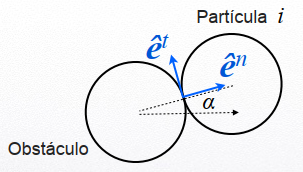
\includegraphics[width=0.7\linewidth]{pic/01-intro/obstacle-collision-diagram}\label{fig:figure-obstacle-collision-diagram}
            \end{figure}
        \end{minipage}
    \end{block}
\end{frame}

